\documentclass[a4paper,12pt]{report}
\linespread{1.5}
\usepackage{geometry}
\geometry{top=3cm,bottom=3cm,left=3.5cm,right=3.5cm} % Impostiamo il valore dei margini.
\usepackage[utf8]{inputenc}
\usepackage{tikz,pgf}
\usepackage{indentfirst}
\usepackage{amsfonts}
\usepackage[english]{babel} %% Abbiamo istruito LaTeX ad usare la lingua italiana.
\usepackage{todonotes}
\usepackage{subfig}
\usepackage{fancyhdr}
\setlength{\parindent}{1cm}
\usepackage{graphicx}
\usepackage{float}
\usepackage{csquotes}
\usepackage{amsmath}
\usepackage{numprint}
\usepackage{pgfplots}
\usepackage{pgfplotstable}
\usepackage{tocbibind}
\usepackage{titling}
\usepackage{wrapfig}
\usepackage{graphics}
%\usepackage{hyperref}
\usepackage[bookmarksopen,bookmarksdepth=2,breaklinks=true,colorlinks=true,urlcolor=black,linkcolor=black]{hyperref}
\graphicspath{{imgs/}} %% cartella dalla quale ricavare le immagini %%

%%%%%%%%%%%%%%%%%%%%%%%%%%%%%%%%%%%%%%%%%%%%%%%%%%%%%%%%%%%%
%% Autore: Fabio Cangeri                                  %%
%% Data: Aprile 2022                                      %%
%%%%%%%%%%%%%%%%%%%%%%%%%%%%%%%%%%%%%%%%%%%%%%%%%%%%%%%%%%%%

\setlength {\marginparwidth }{2cm} 
\pgfplotsset{compat=1.16}

\newenvironment{dedication}
  {\clearpage           % we want a new page
   \thispagestyle{empty}% no header and footer
   \vspace*{\stretch{1}}% some space at the top 
   \itshape             % the text is in italics
   \raggedleft          % flush to the right margin
  }
   {\par % end the paragraph
   \vspace{\stretch{3}} % space at bottom is three times that at the top
   \clearpage           % finish off the page
  }
  

\begin{document}
\begin{titlepage}
\begin{center}
\textbf{\LARGE University of Calabria}\\
\textbf{Department of Mathematics and Computer Science}\\
\vskip 6pt
\hrule
\vskip 8pt
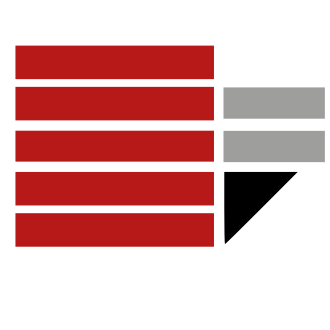
\includegraphics[width=0.13\linewidth]{logo.png}
\vskip 8pt
\textbf{Master’s degree course in Artificial Intelligence and Computer Science}
\vskip 32pt
Machine Learning

\vskip 70pt
{ \huge \bfseries 
    House Price Prediction  
}\\[0.4cm]
\vskip 7pt
Group: Aurora
\vskip 120pt

\begin{tabular}{p{8cm}p{6cm}}
Respective Faculty: & Authors:\\
Prof.~Pasquale Rullo & Fabio Cangeri 249495 \\
Prof.ssa Angelica Liguori & Hilary Tesfay Gebreslassie 241696 \\
 & Hongyu Wang 225200 \\
 & Kidanu Desta Akelom 242386 \\
 & Taiyeba Akter 234600 \\
\end{tabular}

%\begin{tabular}{p{8cm}p{8cm}}
%\includegraphics[width=0.3\linewidth]{imgs/firma.jpg}
%&
%\includegraphics[width=0.3\linewidth]{imgs/firma.jpg}
%\end{tabular}

\vskip 60pt
\hrule
\vskip 6pt
Anno Accademico 2022/2023
\vfill
\end{center}

\end{titlepage}

\begin{dedication}
Namaste
\end{dedication}

%% Corpo della tesi %%

%\chapter*{Sommario} %% In questa zona inseriamo l'abstract del nostro documento. %%
%Inserisci abstract: ...


\tableofcontents
\chapter{Business Understanding}

HousePrice is a tool used for forecasting the selling prices of real estate. When one thinks of a house, from the point of view of the buyers, it is usual to think of purely aesthetic parameters such as a beautiful and large kitchen, a sunny balcony, a guest room without paying much attention to aspects that actually contribute to the price end of the structure, such as the area in which it is located, its proximity to the railway, materials used in the construction, the type of road to access the property, the cadastre of the lot, type of foundations, type of heating, quality of the floors and many other parameters that are generally not considered or are considered as minor. The combination of all these aspects, albeit for some subjects considered of little importance, contribute to a better economic evaluation of the property.



\section{Determine Business Objectives}
Understanding a customer's true goal is as critical for many reasons as understanding the goal you intend to achieve and where to focus your attention in implementation. It is also important to measure the success of the result achieved.

\subsection{Background}
%Record information that is known about the organization’s business situation
Kaggle is an online community of data scientists and machine learning professionals. Enables users to find and publish datasets, explore and build models in a web-based data science environment, work with other data scientists and machine learning engineers, and enter contests to solve data science challenges.

\subsection{Business Objectives}
%(Describe primary objective from a business perspective) 
The goal is to understand which parameters contribute to the market value of a house, which of them allow to increase the economic value more and which less. Formally we have to answer the following question:
\begin{itemize}
    \item What attributes are most related to home price value?
\end{itemize}

\subsection{Business success criteria}
%(Describe the criteria that you’ll see to determine if the project has been successful)
The criterion we use are the relationships that we find between the various attributes that lead to substantial changes in the market value of the house in question.

\section{Assess Situation}
This task involves the resources, requirements, constraints, assumptions, risks, contingencies, glossary of terminology, and the cost-benefit analysis.

\subsection{Inventory of resources}
List of resources available to the project:
\begin{itemize}
\item Personnel: five students of machine learning; 
\item Data: fixed extracts;
\item Computing resources: laptops;
\item Software:
   \begin{itemize}
       \item Programming Language
             \begin{itemize}
                 \item Python: is an interpreted, high-level language with 
dynamic semantics 
             \end{itemize}
        \item Modules (packages)
             \begin{itemize}
                 \item NumPy: is the fundamental package for scientific computing
                 \item Scipy library: provides user-friendly and efficient numerical routines
such as routines for numerical integration and optimization
                 \item Pandas: is a set of structures and data analysis tools
                 \item Scikit-Learn library: is a repository rich of simple and efficient
tools for data mining and data analysis
                 \item Matplotlib: is a plotting library which produces publication
quality figures in a variety of hardcopy formats and interactive
environments across platforms
             \end{itemize}
        \item Sharing Server
             \begin{itemize}
                 \item Jupyter Notebook: is an open-source web application that allows
you to create and share documents that contain live code,
equations, visualization and narrative text
             \end{itemize}
   \end{itemize}
\end{itemize}

\subsection{Requirements, assumptions and constraints}
% List of all requirements of the project, of the assumptions made by the project and list of the constraints on the project
We are not sure that these requirements are the only ones that are relevant in estimating the value of a house, such as the unmentioned plumbing system. Furthermore, the use of new materials on the market, which perhaps have a lower environmental impact but a worse yield than conventional products, are we sure they are evaluated correctly? This of course cannot be verified during data mining nor with any other project-related activity, yet they are worth seeing and mentioning.

\subsection{Risks and contingencies}
\begin{itemize}
\item List of risks or event that might delay the project or cause it to fail: For timing reasons we don't know if we will be able to compare different modeling techniques, in order to find the technique that best describes our problem; We plan to cover at least five models, but we have the unknown factor of time.
\item List of actions to be carried out if the risks arises: In case this problem arises, we are satisfied to be able to conclude a correct analysis and estimation of a modeling technique.
\end{itemize}	

\subsection{Terminology}
%Glossary of terminology relevant to the project) (LATER)
\begin{itemize}
    \item Extreme programming: it is one of the most famous agile methodologies. It's an extreme of iterative development, where multiple versions can be built multiple times in a day, increments are delivered to customers every two weeks. Developers work in pairs, checking each other's work, giving support to do a good job; 
    \item Agile methodology: there is a lot of focus on the code and the product to be delivered as opposed to wasting time on other aspects deemed secondary. The principles of this methodology allow you to create software that works quickly.
    \item Incremental model: this type of model allows you to develop the software in parts, where each part adds features that are requested by the customer.
\end{itemize}

\subsection{Costs and benefits}
%A cost-benefit analysis which compares the costs of the project with the potential benefits
This project involves a more objective assessment of the property than an assessment, albeit made by a person who has gained some experience, by eye and therefore in a subjective way. Very often, some properties have disproportionate prices as there is no rigid guideline to follow in order to estimate a property but the real estate agencies themselves take care of making estimates according to parameters that are ephemeral compared to those considered by the HousePrice system.



\section{Determine Data Mining Goals}
A business goal states objectives in business terminology while a data mining goal states project objectives in technical terms.

\subsection{Data mining Goals}
%(Describe the intended outputs that enables the achievement of the project objectives) 
The goal is to create a tool capable of estimating new properties that will be put on the market, understanding the importance of the parameters that contribute to the economic evaluation of the property, in order to have a more accurate estimate of the value of the property based on the parameters that allow its value to be surveyed. For each property there is no right or wrong answer to its market value and it is not even possible to make a comparison with other properties present, albeit close to rent, as each property has different characteristics from each other.

\subsection{Data mining Success Criteria}
%(Define the criteria for a successful outcome) 
The criterion we use to determine if our project is successful is to find the best valuation model to rank the final price of each house.

\section{Produce Project Plan}
Description of the plan envisaged to achieve the data mining objectives and thereby achieve the business objectives.

\subsection{Project Plan}
%(List of the stages to be executed, together with their duration, resources required, inputs, outputs and dependencies)

\begin{figure}[t]
    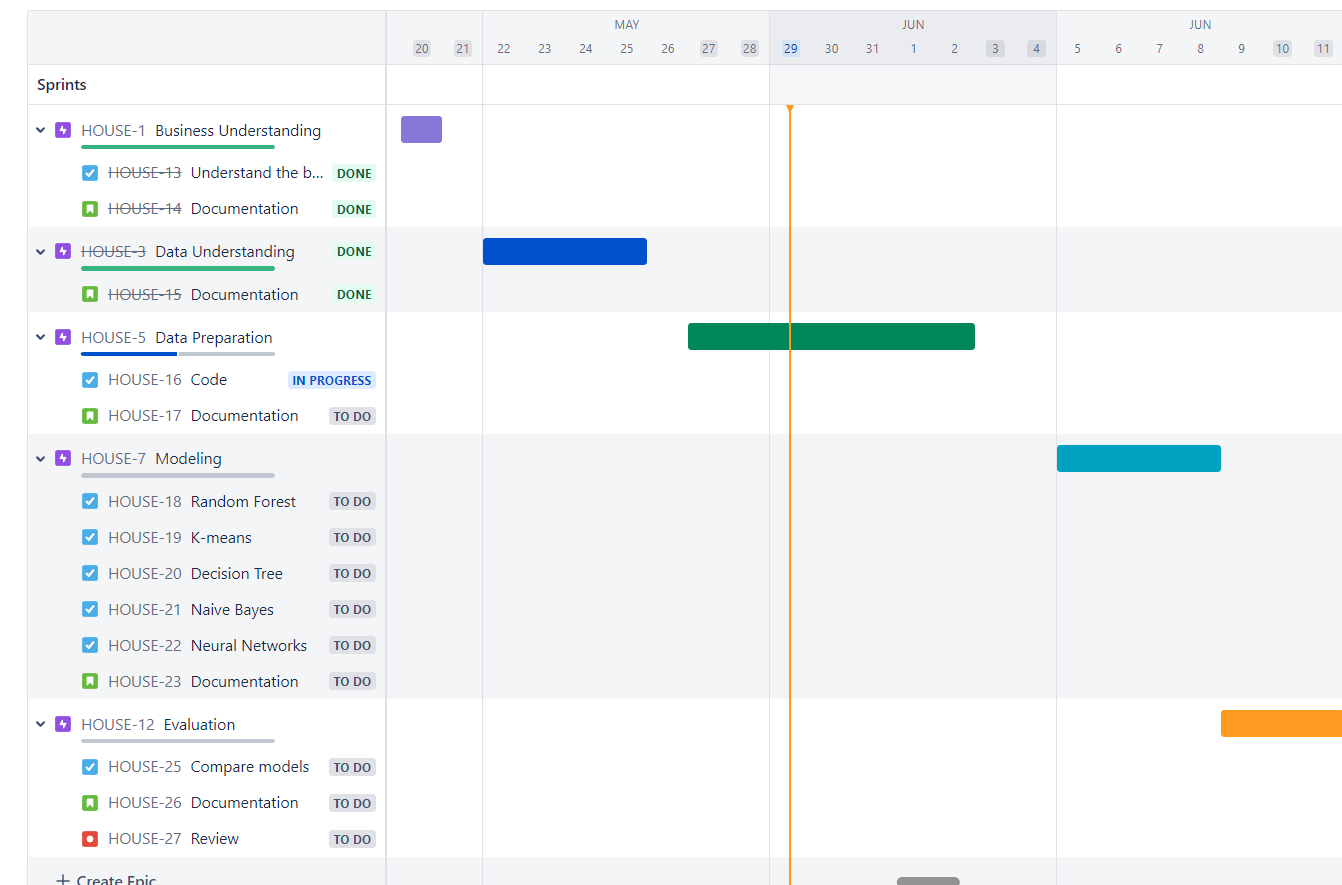
\includegraphics[scale=0.45]{imgs/jira_schedule.png}
    \centering
    \caption{Jira schedule}
    \hrulefill\vspace{15pt}\par
\end{figure}

The phases that we are going to perform by dividing the work by trying different methodologies in order to create a model as close as possible to the training set provided. Initially we plan to work together to get to know each other better, understand the individual potentials of each of us and to understand and respect the objective of the project. Subsequently, let's assume that we can work according to the methodology 'Extreme Programming'. Each of us has assumed control of a part to hold ourselves accountable.
We plan to spend our time, as is possible see in the figure 1.1, distributing the hours in this way:
\begin{itemize}
\item Business Understanding: 5\% of total hours;
\item Data Understanding: 10\%;
\item Data Preparation: 75\%; 
\item Modeling: 5\%;
\item Evaluation: 5\%.
\end{itemize}

\subsection{Initial Assessment of Tools and
Techniques}
%Select data mining tool that supports various methods for different stages
The data mining tool that we use to supports various methods for different stages is Scikit-learn library. We used it to supports, supervised, unsupervised learning, model fitting, data preprocessing, model selection, model evaluation, and many other utilities.
\chapter{Data Understanding}
\chapter{Data Preparation}

\section{Select Data}

\subsection{Rationale for inclusion/exclusion}
% List the data to be included/excluded and the reasons for these decisions

We have utilized a Python code that includes a function for data preparation by calculating the entropy of a set of labels. The entropy function is essential for various learning tasks and provides valuable insights for feature selection, model training, and decision-making processes.
The entropy calculation is performed using the formula in figure 3.1, where:
\begin{itemize}
    \item \textbf{Labels} refer to the set of labels;
    \item \textbf{n} is the number of distinct labels;
    \item \textbf{pi} represents the probability of each label \textbf{i} within the set.
\end{itemize}
To calculate the entropy, figure 3.2, the function first converts the labels to integer indices, ensuring compatibility with subsequent calculations. It then computes the probabilities of each label by counting their occurrences and dividing by the total number of labels. Finally, the entropy is calculated using the probabilities and the logarithmic function.
This data preparation step is valuable for understanding the diversity and distribution of labels within the dataset. By assessing the entropy, informed decisions can be made regarding data preprocessing, feature selection, and modeling strategies. An entropy value of 0 indicates perfect purity, where all labels in the set are the same. Conversely, higher entropy values indicate a more diverse distribution of labels and higher uncertainty in predicting the class or category of an instance.

\begin{figure}%[!h]
\begin{center}
    
\includegraphics[scale=0.45]{imgs/entropy.png}
    \centering
    \caption{Entropy formula}
    \vspace{15pt}
    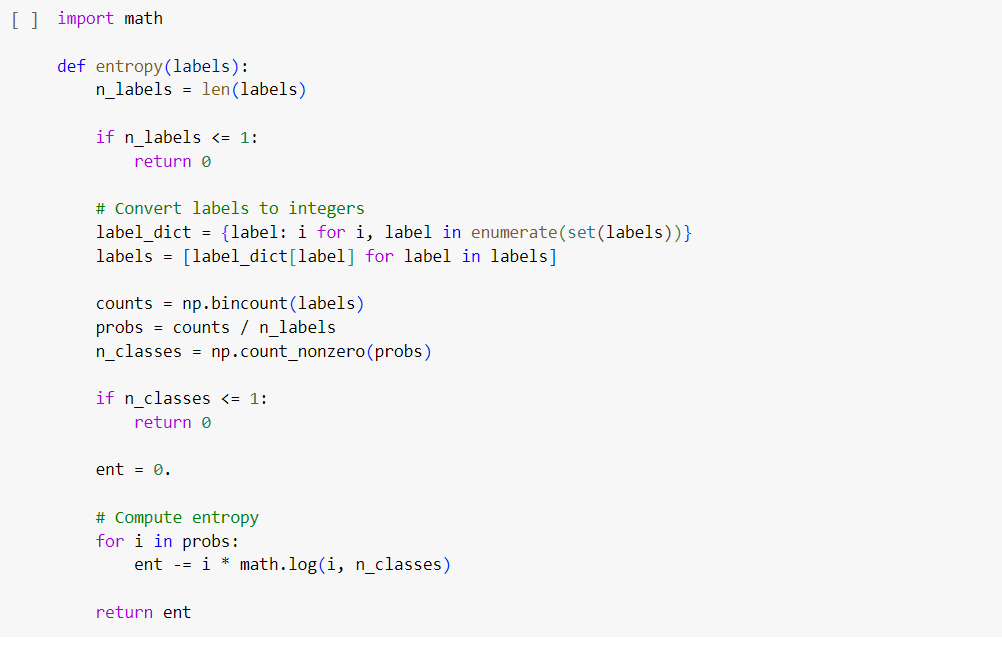
\includegraphics[scale=0.45]{imgs/entropy_function.png}
    \centering
    \caption{Entropy function}
\end{center}
\hrulefill\vspace{15pt}\par
\end{figure}

Based on the above exploratory analysis, a feature subset selection process was conducted to remove features that exhibited low entropy values, figure 3.3. The entropy threshold of 0.2 was set to identify features with limited information gain or relevance to the dataset.
The process involved iterating over each column in the 'housePrice' DataFrame and calculating the entropy for each column using the previously defined entropy() function. If the entropy of a column was found to be below the threshold, it was considered an indicator of low information gain or redundancy.
The selected features, identified through their low entropy values, were printed out, and the 'drop()' method was utilized to remove them from the 'housePrice' DataFrame. This was done by specifying the column name and using the axis=1 parameter to drop the features along the columns.
By removing irrelevant or redundant features, the dimensionality of the dataset was reduced, which can enhance the efficiency and performance of subsequent machine learning algorithms. The aim of this feature selection process was to retain only the most informative features that contribute significantly to the predictive power of the dataset.
This reduction offers advantages such as improved computational efficiency, reduced risk of overfitting, and enhanced interpretability of models. By focusing on the most important predictors, the selected subset may lead to more accurate predictions and better generalization to unseen data.
After performing the feature subset selection, the original data frame, which initially consisted of 81 columns, was reduced to 64 columns, retaining the most informative features.

\begin{figure}[t]
    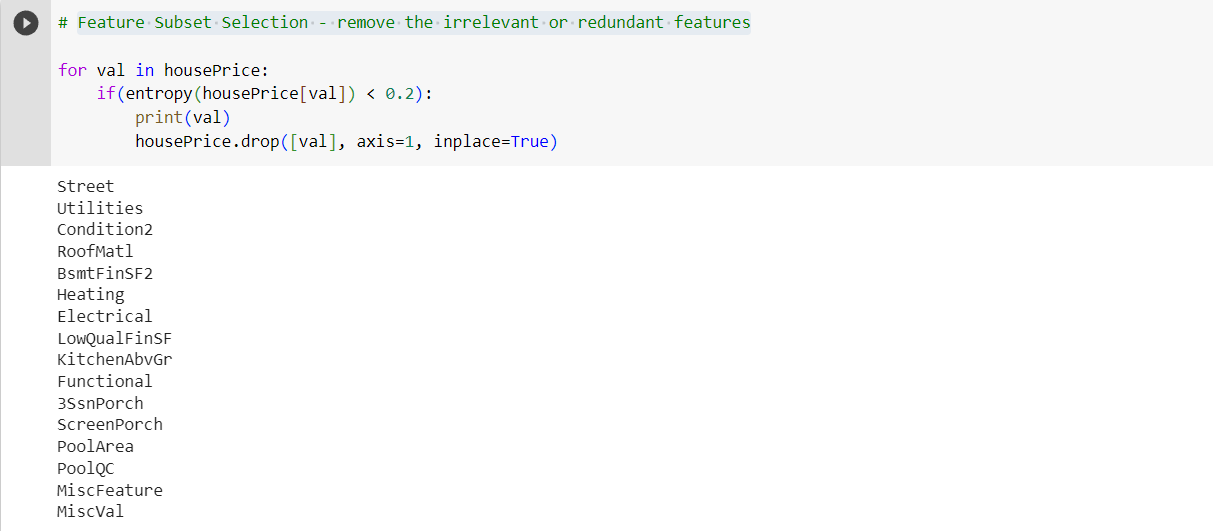
\includegraphics[scale=0.45]{imgs/feature_subset_selection.png}
    \centering
    \caption{Feature subset selection}
    \hrulefill\vspace{15pt}\par
\end{figure}

\section{Clean Data}

Since we have data understanding, we will now do data cleaning.  Data cleaning step is a very crucial step for reliable and better performance of our model in machine learning. In our data cleaning we have identified and removed noises in order to ensure that we have the accurate dataset for analysis. Checked for duplication and missing value on the given dataset of each attribute. 

\subsection{Data Cleaning Report}
% Describe what decisions and actions you took to address data quality problems

\begin{figure}[t]
    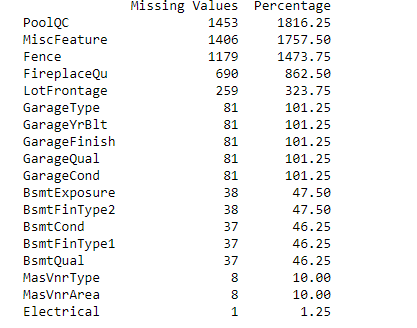
\includegraphics[scale=0.55]{imgs/missing_value.png}
    \centering
    \caption{Missing value}
    \hrulefill\vspace{15pt}\par
\end{figure}

We have 1460 unique Id in our dataset. We have used this Id in order to identify in case of duplicated instances in our dataset. Our dataset is consisting of 1460 rows and 81 columns. Each row Id were unique hence we were able to not use Id for our training set.

Given that for the attribute Alley with value of NA were considered as a value of object and not a missing value, figure 3.4, for the rest of the dataset we have found 18 columns that have missing value, in which the sum value of missing value or null was above 0. In the fig below we can see the attributes in which their missing value was not 0, PoolQC, MiscFeature and Fence having to large amount of missing value.
To remove the missing value, we have replaced the null value with mean value taking example LotFrontafe, GarafeYrBlt and MasVnrArea columns.

We have checked that there is:
\begin{itemize}
    \item Negative value: in our data set we do not have negative values.;
    \item No negative value and now we check if there is duplication, but we have non-unique value on our dataset except the attribute of Id;
    \item Out-of-range values: the attributes we didn’t consider while training out mode are Id and SalePrice. SalePrice was determined by the added PriceLabel, and we did not use it for our training data only when labelling the value on PriceLabel.;
    \item Inconsistency: we didn’t have data inconsistencies;
    \item Duplicate: We have checked that there is no negative value and now we check if there is duplication, but we have non-unique value on our dataset except the attribute of Id. Hence, we have not found any duplication.
\end{itemize}
     

\section{Construct Data}

\subsection{Derived attributes}
% New attriutes constructed from one or more existing attributes

To gain insights into trends and patterns based on the construction year, the 'housePrice' DataFrame is grouped using the 'YearBuilt' column. This grouping creates separate subsets of data for each unique year. The mean() method is then applied to calculate the average values for each numerical attribute within each group. This provides a new DataFrame displaying the average attribute values grouped by the construction year.
By calculating the mean values for each attribute, we can analyze the central tendency or average level of different attributes for each year. This allows us to identify potential relationships or dependencies between the construction year and other quantitative attributes in the dataset.
This information can aid in making informed decisions, such as identifying important features for predictive modeling or understanding the impact of time on attribute values.

\begin{figure}[t]
    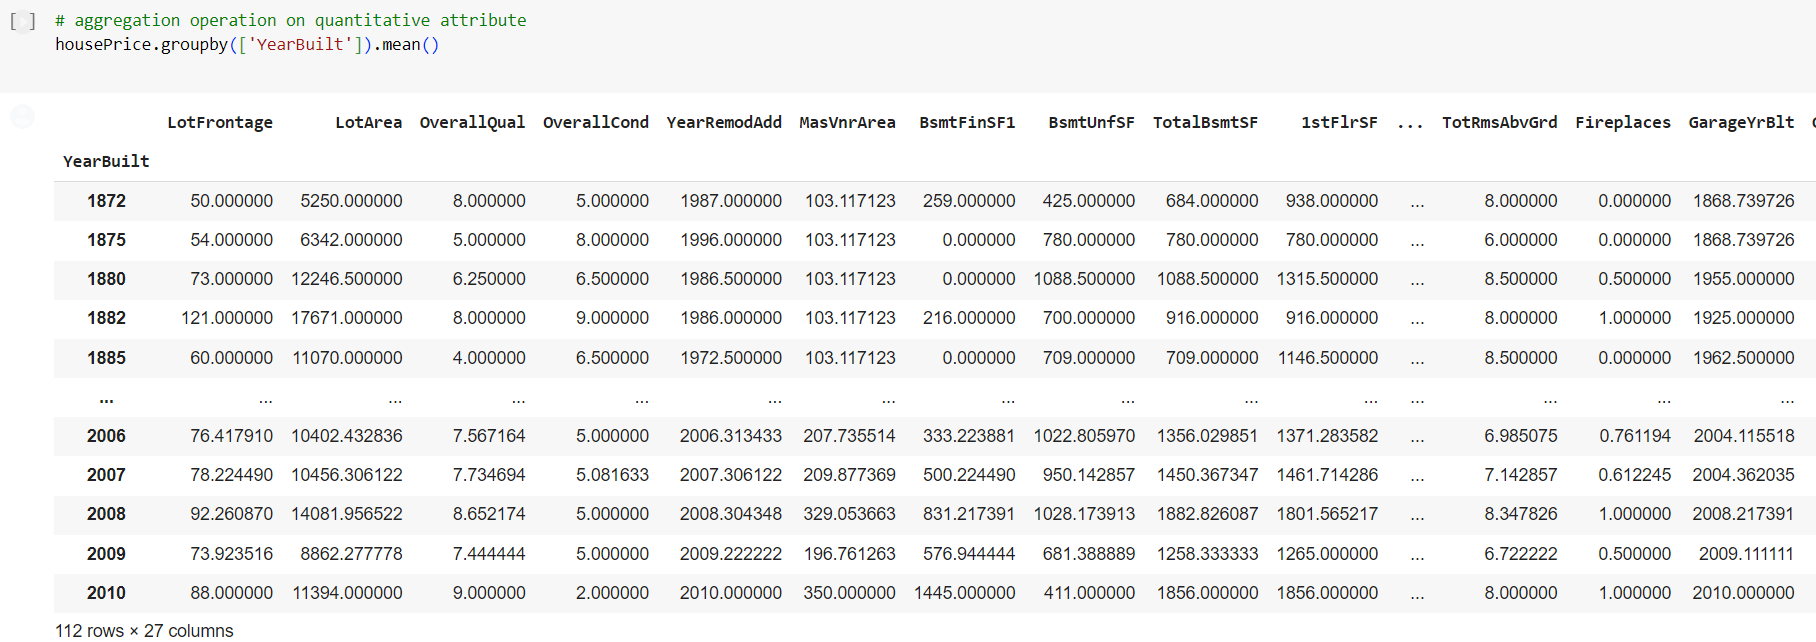
\includegraphics[scale=0.35]{imgs/aggregate_operation.png}
    \centering
    \caption{Aggregate operation}
    \hrulefill\vspace{15pt}\par
\end{figure}


\subsection{Generated records}
% Describe the creation of any completely new records

To capture important information more efficiently in the dataset, a feature creation process was employed by combining the 'OverallQual' and 'OverallCond' attributes. The goal was to generate a new attribute that captures a consolidated measure of the overall quality and condition of the houses. By combining the 'OverallQual' and 'OverallCond' attributes using the addition operator, a new attribute called 'OverallQualCond' was created. This composite feature aims to provide a more comprehensive assessment of each house's overall state, considering both material and finish quality and overall condition.
Following the creation of the 'OverallQualCond' feature, the original 'OverallQual' and 'OverallCond' attributes were dropped from the 'housePrice' DataFrame. This step was taken to remove redundancy and potential multicollinearity issues that could arise from using highly correlated attributes in subsequent modeling tasks, figure 3.5.
As a result of this feature creation process, the modified 'housePrice' DataFrame now includes the newly created 'OverallQualCond' feature while no longer containing the original 'OverallQual' and 'OverallCond' attributes. The inclusion of the 'OverallQualCond' feature provides a consolidated representation of each house's overall quality and condition, potentially offering a more informative and concise feature for analysis and modeling purposes.

\section{Integrate Data}

\subsection{Merged Data}
% To join toghetere two or more tables that have different information about the same objects

In this stage of the data preparation process, there was no need to merge data from multiple sources. The project solely relies on a single dataset, and therefore, there was no requirement to combine or integrate data from different sources.

\begin{figure}%[!h]
\begin{center}
    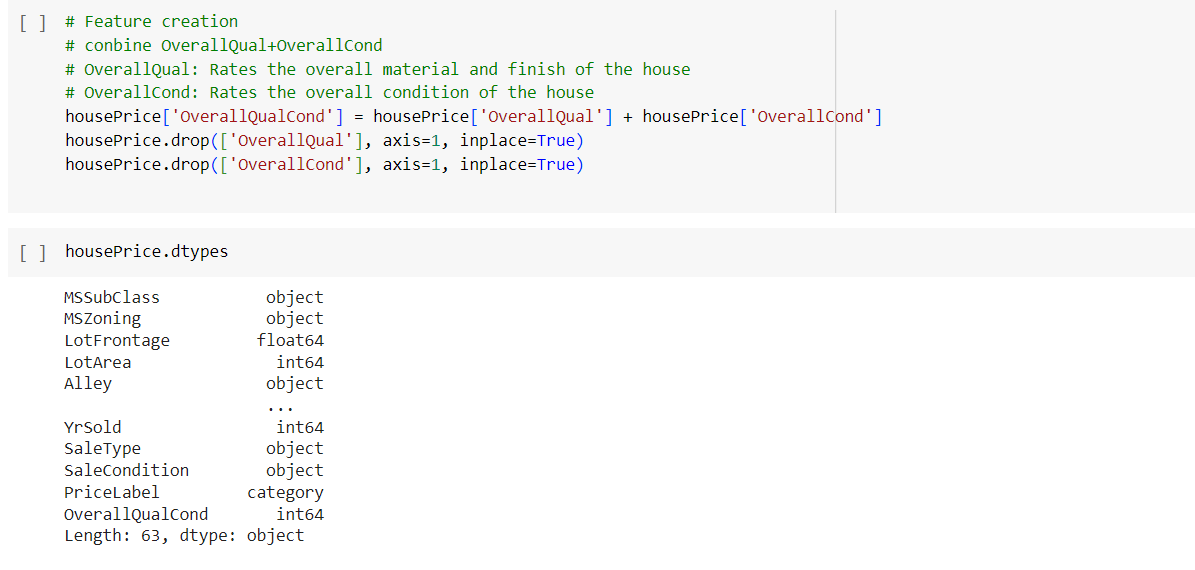
\includegraphics[scale=0.5]{imgs/feature_creation.png}
    \centering
    \caption{Feature creation}
    \vspace{15pt}
    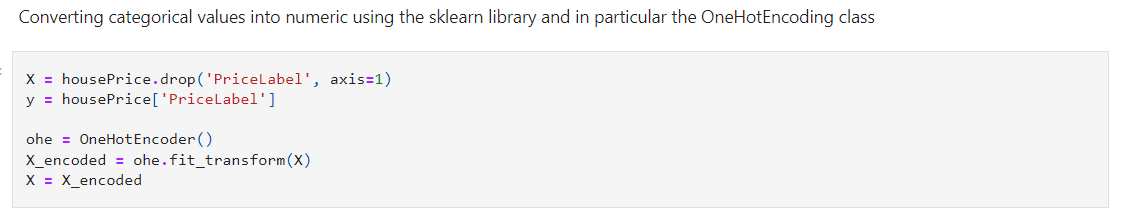
\includegraphics[scale=0.5]{imgs/one_hot_encoder.png}
    \centering
    \caption{OneHotEncoder}
\end{center}
\hrulefill\vspace{15pt}\par
\end{figure}


\section{Format Data}

\subsection{Reformatted Data}
% To satisfy the modeling tool requirementes

In this stage, we have used OneHotEncoder class in scikit-learn for converting our categorical variables into a binary vector representation, figure 3.7, where each category is represented by a separate binary column. This allows the algorithms we have used to consider the presence or absence of each category as a separate feature.
Moreover, the resulting encoded features allow the models to handle categorical data and incorporate it into the learning process, improving the model's ability to capture patterns and make accurate predictions.
\chapter{Modeling}

\section{Select Modeling Tecnique}

\subsection{Modeling Technique}
% Document the modeling technique that you’ll be using
Random Forest Tree: Random forest is an ensemble learning method for classification, regression and other tasks that operate by constructing a multitude of decision trees at training time and outputting the class that is the mode of the classes (classification) or mean prediction (regression) of the individual trees. Random forest is known for its accuracy and robustness to noise and outliers.

Neural Network: Neural networks are a set of algorithms that are modeled after the human brain and are designed to recognize patterns. Neural networks are used for image recognition, speech recognition, natural language processing, and many other applications. Neural networks are known for their ability to learn from data and generalize to new data.

Adaboost: AdaBoost is an ensemble learning method that combines multiple weak classifiers to create a strong classifier. AdaBoost is used for classification problems and is known for its high accuracy and robustness to noise.

Naive Bayes: Naive Bayes is a probabilistic algorithm that is based on Bayes’ theorem. Naive Bayes is used for classification problems and is known for its simplicity and speed.

Decision Tree: A decision tree is a supervised learning algorithm that is used for classification and regression modeling. It is a method used for predictive modeling, so these trees are used to either classify data or predict what will come next. Decision trees in machine learning can either be classification trees or regression trees. 

\subsection{Modeling Assumptions}
% Record any assumptions about the data that are necessary for the modeling techniques
Random Forest Tree: Random forest assumes that the data is independent and identically distributed (i.i.d.) and that there are no missing values in the data.

Neural Network: Neural networks assume that the data is linearly separable and that there are no missing values in the data.

Adaboost: AdaBoost assumes that the data is i.i.d. and that there are no missing values in the data.

Naive Bayes: Naive Bayes assumes that the features are independent of each other and that there are no missing values in the data.

Decision Tree: Decision tree is a non-statistical approach that makes no assumptions of the training data or prediction residuals; e.g., no distributional, independence, or constant variance assumptions.


\section{Generate Test Design}

\subsection{Test Design}
% Describe how to divide the available dataset into training, test and validation datasets
Generating a test design is an important step in evaluating the performance of modeling techniques. To generate a test design, one needs to define the objective and scope of the test, select the test data, define the performance metrics, and define the procedure for conducting the test.

\section{Build Model}  

\subsection{Random Forest Tree}



We used the sklearn.ensemble library for the Random Forest Tree model. We also employed 5-fold cross-validation to train the model. Finally, we saved the best model out of five and used it for evaluation.
We evaluated the model using different criteria and plotted the Confusion Matrix on Figure~\ref{cmRFT}. The table~\ref{tableRFT} shows the scores for each criterion.
  

\begin{table}[H]  \centering  
    \begin{tabular}{@{}lllll@{}}
    \toprule
    \multicolumn{5}{c}{Random Forest Tree}                 \\ \midrule
    \multicolumn{5}{l}{Accuracy: 0.8767123287671232}       \\\midrule
                 & precision & recall & f1-score & support \\
    HIGH         & 0.90      & 0.47   & 0.62     & 19      \\ 
    LOW          & 0.86      & 0.96   & 0.91     & 125     \\
    MEDIUM       & 0.89      & 0.86   & 0.88     & 148     \\
    accuracy     &           &        & 0.88     & 292     \\
    macro avg    & 0.88      & 0.76   & 0.80     & 292     \\
    weighted avg & 0.88      & 0.88   & 0.87     & 292     \\ \bottomrule
    \end{tabular}
    \caption{Classification Report of Random Forest}
    \label{tableRFT}
\end{table}


\begin{figure}[H]
    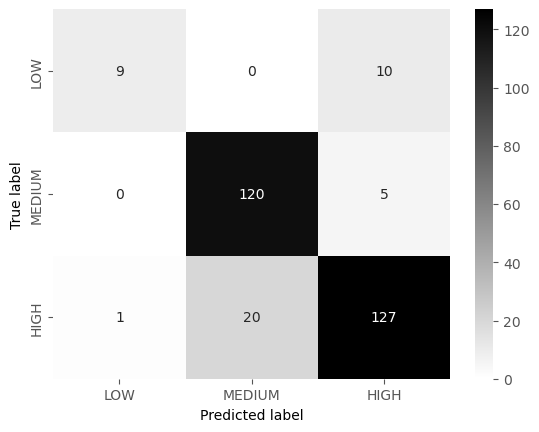
\includegraphics[scale=0.7]{imgs/rft_cm}
    \centering
    \caption{Confusion Matrix of Random Forest Tree}
    \label{cmRFT}
\end{figure}


\subsection{Neural Network}

As for Neural Network, We choose the library of MLPClassifier which is part of the Scikit-learn library in Python , The MLPClassifier is a neural network algorithm used for classification tasks. Some parameters are used in this model. The hidden\_layer\_sizes parameter specifies the number of neurons in each layer of the neural network. In this case, there are two hidden layers with 5 neurons each. The activation parameter specifies the activation function used in each neuron. In this case, the ReLU activation function is used. The random\_state parameter is used to initialize the random number generator for reproducibility. The alpha parameter is used for regularization to prevent overfitting. The max\_iter parameter specifies the maximum number of iterations for the solver to converge. The solver parameter specifies the optimization algorithm used to minimize the loss function. In this case, the stochastic gradient descent (SGD) algorithm is used. The tol parameter specifies the tolerance for stopping criteria. The learning\_rate\_init parameter specifies the initial learning rate used by the optimizer 1. 
Here also plot the confusion Matrix~\ref*{cmNN} and the result of evaluated table~\ref*{tableNN}.


\begin{table}[H]\centering
    \begin{tabular}{@{}lllll@{}}
    \toprule
    \multicolumn{5}{c}{Neural Network}                 \\ \midrule
    \multicolumn{5}{l}{Accuracy: 0.84}       \\\midrule
                 & precision & recall & f1-score & support \\
    HIGH         & 0.56      & 0.72   & 0.63     & 25      \\ 
    LOW          & 0.82      & 0.90   & 0.86     & 173     \\
    MEDIUM       & 0.89      & 0.80   & 0.84     & 240     \\
    accuracy     &           &        & 0.84     & 438     \\
    macro avg    & 0.76      & 0.81   & 0.78     & 438     \\
    weighted avg & 0.84      & 0.84   & 0.84     & 438     \\ \bottomrule
    \end{tabular}
    \caption{Classification Report of Neural Network}
    \label{tableNN}
\end{table}

\begin{figure}[H]
    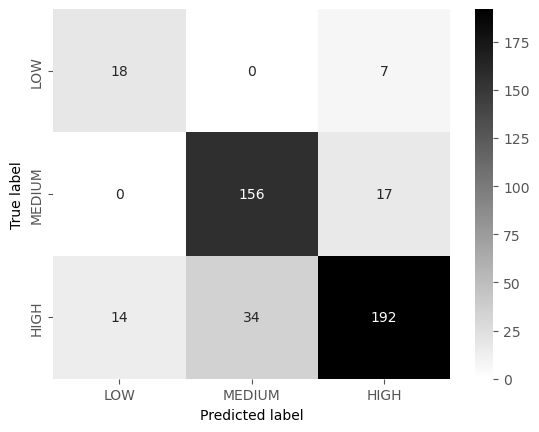
\includegraphics[scale=0.7]{imgs/nn_cm}
    \centering
    \caption{Confusion Matrix of Neural Network}
    \label{cmNN}
\end{figure}

\subsection{AdaBoost}

For the AdaBoostClassifier, it is an ensemble learning method that combines multiple weak learners to create a strong classifier. The n\_estimators parameter specifies the number of weak learners to train iteratively. The learning\_rate parameter contributes to the weights of weak learners and uses 1 as a default value.
The Confusion Matrix shows at~\ref*{cmadb} and the evaluation table shows at~\ref*{tableADB}.

\begin{table}[H]\centering
    \begin{tabular}{@{}lllll@{}}
    \toprule
    \multicolumn{5}{c}{Adaboost}                 \\ \midrule
    \multicolumn{5}{l}{Accuracy:  0.8333333333333334}       \\\midrule
                 & precision & recall & f1-score & support \\
    HIGH         & 0.61      & 0.76   & 0.68     & 25      \\ 
    LOW          & 0.80      & 0.90   & 0.85     & 173     \\
    MEDIUM       & 0.89      & 0.79   & 0.84     & 240     \\
    accuracy     &           &        & 0.11     & 438     \\
    macro avg    & 0.77      & 0.82   & 0.79     & 438     \\
    weighted avg & 0.84      & 0.83   & 0.83     & 438     \\ \bottomrule
    \end{tabular}
    \caption{Classification Report of Adaboost}
    \label{tableADB}
    \end{table}

    \begin{figure}[H]
        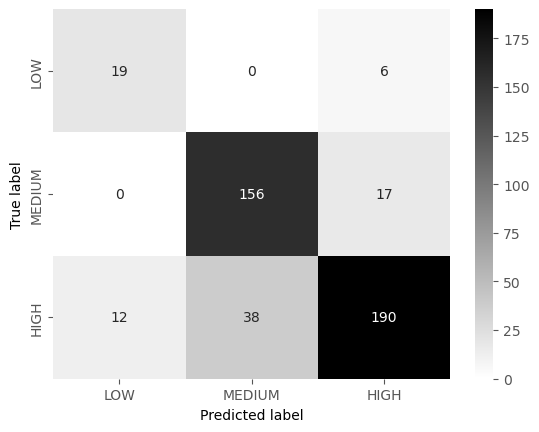
\includegraphics[scale=0.7]{imgs/adb_cm}
        \centering
        \caption{Confusion Matrix of Adaboost}
        \label{cmadb}
    \end{figure}


\subsection{Naive Bayes}

The project also uses the Gaussian Naive Bayes algorithm to train a model on the training data. The Gaussian Naive Bayes algorithm is a type of Naive Bayes algorithm that assumes that all features are independent of each other and follow a Gaussian distribution. It is used for classification problems where the input variables are continuous.

The GaussianNB() function from the sklearn.naive\_bayes module is used to create an instance of the Gaussian Naive Bayes algorithm. The instance is then trained on the training data using the fit() method.

the result of Confusion Matrix~\ref*{cmnb} and evaluation table~\ref*{tablenb} list here.


\begin{table}[H]\centering
    \begin{tabular}{@{}lllll@{}}
    \toprule
    \multicolumn{5}{c}{Naive Bayes}                 \\ \midrule
    \multicolumn{5}{l}{Accuracy: 0.8427}       \\\midrule
                 & precision & recall & f1-score & support \\
    HIGH         & 0.46      & 0.24   & 0.32     & 25      \\ 
    LOW          & 0.69      & 0.77   & 0.73     & 173     \\
    MEDIUM       & 0.76      & 0.74   & 0.75     & 240     \\
    accuracy     &           &        & 0.72     & 438     \\
    macro avg    & 0.64      & 0.58   & 0.60     & 438     \\
    weighted avg & 0.72      & 0.72   & 0.72     & 438     \\ \bottomrule
    \end{tabular}
    \caption{Classification Report of Naive Bayes}
    \label{tablenb}
    \end{table}




\begin{figure}[H]
    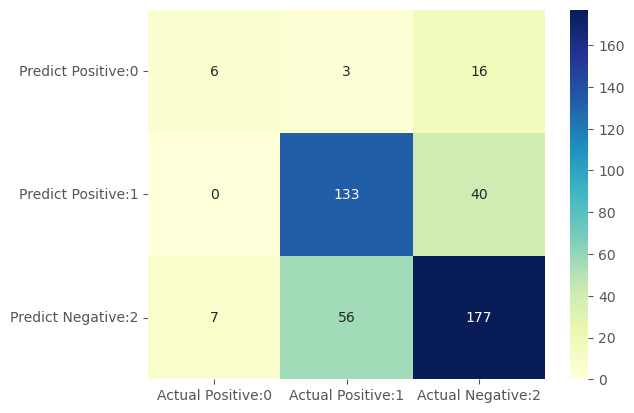
\includegraphics[scale=0.7]{imgs/nb_cm}
    \centering
    \caption{Confusion Matrix of Naive Bayes}
    \label{cmnb}
\end{figure}

\subsection{Decision Tree} 

The DecisionTreeClassifier is a class in the sklearn.tree module of the Python Scikit-learn library. It is used to create a decision tree classifier which is a predictive model that can be used for both classification and regression problems. The criterion parameter specifies the function to measure the quality of a split. In this case, we use the supported criteria is “gini” for the Gini impurity.
Confusion Matrix~\ref{cmdt} and Classification Report of Decision Tree~\ref{tabledt}.
\begin{table}[H]\centering
    \begin{tabular}{@{}lllll@{}}
    \toprule
    \multicolumn{5}{c}{Decision Tree}                 \\ \midrule
    \multicolumn{5}{l}{Accuracy: 0.7990867579908676}       \\\midrule
                 & precision & recall & f1-score & support \\
    HIGH         & 0.49      & 0.68   & 0.57     & 25      \\ 
    LOW          & 0.79      & 0.87   & 0.83     & 173     \\
    MEDIUM       & 0.86      & 0.76   & 0.81     & 240     \\
    accuracy     &           &        & 0.80     & 438     \\
    macro avg    & 0.71      & 0.77   & 0.73     & 438     \\
    weighted avg & 0.81      & 0.80   & 0.80     & 438     \\ \bottomrule
    \end{tabular}
    \caption{Classification Report of Decision Tree}
    \label{tabledt}
    \end{table}

    \begin{figure}[H]
        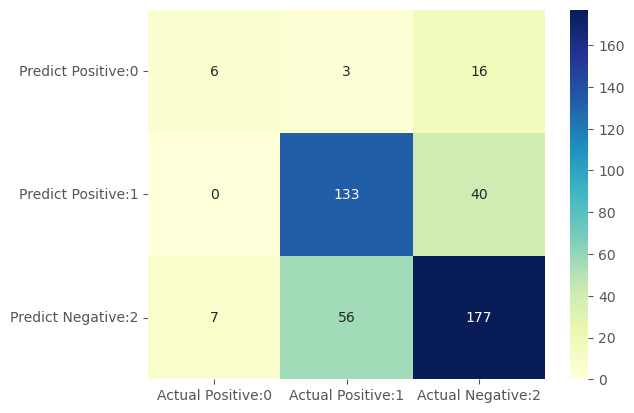
\includegraphics[scale=0.7]{imgs/nb_cm}
        \centering
        \caption{Confusion Matrix of Decision Tree}
        \label{cmdt}
    \end{figure}
\chapter{Evaluation}
\section{Evaluate Results}

In the evaluation phase, we respond exhaustively to the company objectives required of us. Since we believe that the goal is very generic, we took the liberty of putting forward a first development model to see if this already satisfies our client's request; A more focused analysis of the business objective is seen by our team as a possible future direction of the project.

\subsection{Assessment of Data Mining Results}
% Summarize assessment results in terms of business success criteria

\begin{figure}%[!h]
\begin{center}
\begin{minipage}{.5\textwidth}
  \centering
  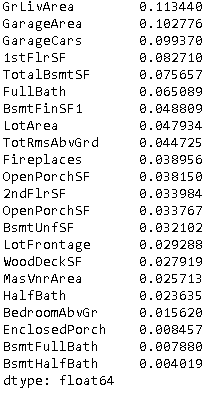
\includegraphics[width=0.7\linewidth]{imgs/feature_scores_numerical.png}
  \captionof{figure}{Feature importance - only numerical}
\end{minipage}%
\begin{minipage}{.5\textwidth}
  \centering
  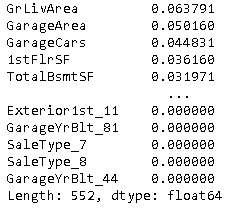
\includegraphics[width=0.7\linewidth]{imgs/feature_scores_categorical.png}
  \captionof{figure}{Feature importance}
  \vspace{50pt}
  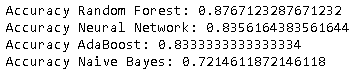
\includegraphics[width=0.7\linewidth]{imgs/accuracy_models.png}
  \captionof{figure}{Accuracy models}
\end{minipage}
\end{center}
\hrulefill\vspace{15pt}\par
\end{figure}

We can answer the following question posed to us:
\\
\emph{What attributes are most related to home price value?}

To answer the question we used the importance of the attributes calculated on the random forest model. It is shown in figure 5.1, for the numerical attributes only, and in figure 5.2 for all the attributes that make up the training set. This calculation is based on the effect that each attribute has on the prediction of the final price; a higher score means that the specific function has a greater effect on the model used to predict a particular variable. 

\subsection{Approved Models}
% After assessing models with respect to business success criteria, the generated models that meet the selected criteria become the approved model

The analysis we have conducted shows that all the models we have developed have a good match in terms of accuracy, as visible in figure 5.2, with the test set. We believe we can predict the price of a home based on its features with reasonable accuracy. 

\begin{figure}[t]
\begin{center}
\begin{minipage}{.5\textwidth}
  \centering
  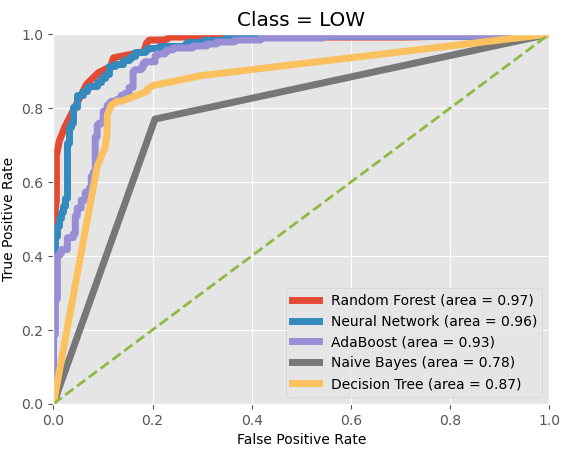
\includegraphics[width=0.9\linewidth]{imgs/roc_low.png}
  \captionof{figure}{ROC Curve Low}
\end{minipage}%
\begin{minipage}{.5\textwidth}
  \centering
  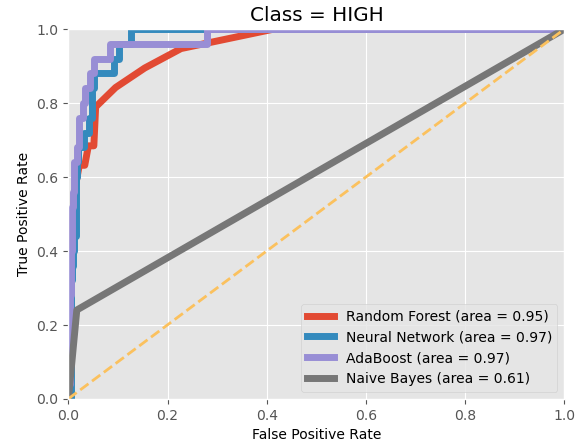
\includegraphics[width=0.9\linewidth]{imgs/roc_high.png}
  \captionof{figure}{ROC Curve High}
\end{minipage}
\end{center}
\end{figure}

\begin{figure}[t]
    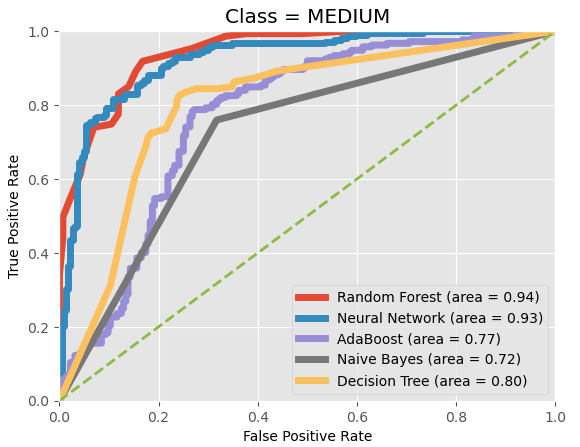
\includegraphics[scale=0.45]{imgs/roc_medium.png}
    \centering
    \caption{ROC Curve Medium}
    \hrulefill\vspace{15pt}\par
\end{figure}

We compared the performance of the models used using different metrics, such as the ROC curve from figure 5.3 to 5.5, which showed a certain score similarity between the Neural Network and the Random Forest model. However, the use of other metrics, such as the confusion matrix, has shed light on the model through accuracy and recall. In conclusion we can say that Random Forest model and Neural Network model are both considered as best machine
learning model for this work. 

\section{Review Process}
% Summarize the process review and highlight activities that have been missed and those that should be repeated

In the project review we checked all the activities carried out so far. Although satisfied with the overall project completed, we continue to ask ourselves whether the analysis carried out to find the most relevant attributes in estimating the price of a house is sufficient or not to start a modernization of the models. However, we believe that a more in-depth analysis, under various profiles, could be the subject of future insights. Regarding the model made, we always ask ourselves the question of whether better accuracy can be achieved. Are we sure we can't do better?

\section{Determine Next Steps}

For the next steps, we have found two that are completely different. One step would allow us to move forward with the software development process, moving to the Deployment phase, while the other step would require a review of the completed phases. In the realization of our software we have followed an incremental model.

\subsection{List of Possible Actions}
% List the potential further actions
\begin{itemize}
    \item Does calculating attribute importance using other models yield the same result?
    \item In the light of what has been discovered, would eliminating the "useless" features lead to an improvement both in terms of model timing, since its dimensionality is reduced, and in terms of performance?
    \item Are we sure these "useless" features don't change over the years? In this case, is still correct removed they to improve our model?
    \item Should we proceed with the deployment?
\end{itemize}

\subsection{Decision}
%  Describe the decision as to how to proceed

To extend the research of the importance of the attributes it is sufficient to use the other models that we have used in the realization of the project. Although these models are not as accurate as the random forest, they could be a valid yardstick with the results obtained.
Removing unnecessary features is a design variant that could make the software grow in terms of quality, however, our team strongly believes that unnecessary parameters will change over the years (for example with the discovery of a material deemed good for construction and subsequently not). However, a hybrid solution of elimination could be adopted, as some parameters tend to never go out of style, such as a large house.
You should talk to the company to understand in which of the two directions they intend to move.
%\chapter{Bibliografia}

%[1] Android Developers. \\
%URL: \url{https://developer.android.com}\\

%Eliminare/Aggiungere/Personalizzare i capitolo nella cartella "capitoli"

%\chapter*{Conclusioni} In questo modo non comparirà dell'indice

%\begin{thebibliography}{100} %% 100 rappresenta il n° massimo di voci all'interno della bibliografia: può essere modificato a vostro piacimento. %%
%\bibitem{[1]:}
%\bibitem{[2]:}
%\bibitem{[3]:}
%\bibitem{[4]:}

%\end{thebibliography}

%\chapter*{Ringraziamenti}
%Inserisci frasi sdolcinate: ...
\end{document}
